% 9장 강건성. 0016 · 0017 · 0020 · 0027 · 0028 · 0030 · 0031

\section{강건성}

이 장은 \textbf{결과를 무너뜨리려는 시도}를 모은 것이다. 일곱 가지를 걸었고, 그중
둘은 ``걸어 봤더니 가릴 수 없다''가 결과였다. 그것도 적는다.

\subsection{위약 검정}

위약 검정은 효과를 재는 것이 아니라 \textbf{측정 도구를 검사}하는 것이다. 아무 일도
없었어야 할 자리에 같은 추정을 돌려 0이 나오는지 본다. 0이 나오지 않으면 그 설계가
\textbf{없는 효과도 만들어 낸다}는 뜻이다.

필요가 생긴 이유가 있다(0016). 고가 처치동은 처치 전에 이미 특이했다 --- 법정동
$\times$ 사건월 칸당 평균 42.2건으로 고가 통제동(15.7건)의 2.7배였고 사후에
10.3 대 8.7로 수렴한다. \textbf{`원래 활발하던 곳이 평균으로 돌아온 것'과 `규제가
거래를 막은 것'은 자료에서 같게 보인다.}

이 절의 숫자는 \textbf{사후 24개월을 하나로 묶은 이중차분}($-33.5\%$)이며, 5장의
직후 효과와 \textbf{다른 값}이다. 섞어 쓰면 안 된다.

% 자동 생성 — scripts/build_tables.py. 손으로 고치지 않는다.
% 출처: output/results/13_placebo.json : A_가짜사건일
\begin{table}[htbp]
  \centering
  \caption{위약 --- 지정이 없던 날을 사건일로 두고 같은 추정을 돌렸다.}
  \label{tab:placebo-date}
  \begin{tabular}{lrr}
    \toprule
    \textbf{가짜 사건일} & \textbf{효과 (\%)} & \textbf{$p$} \\
    \midrule
    2013-06-23 & -5.0 & 0.699 \\
    2014-06-23 & -4.3 & 0.663 \\
    2015-06-23 & -9.7 & 0.088 \\
    2016-06-23 & -21.5 & 0.021 \\
    2017-06-23 & -16.6 & 0.049 \\
    2023-06-23 & -2.3 & 0.836 \\
    2024-06-23 & -1.9 & 0.864 \\
    \bottomrule
  \end{tabular}

  \begin{minipage}{\linewidth}\footnotesize
  \textit{주.} 진짜($-33.5\%$)가 가짜 최대($-21.5\%$)의 1.5배다. 다만 2016·2017 창에는 8·2 와 9·13 대책이 들어 있어 완전한 위약이 아니다.
  \end{minipage}
\end{table}


\begin{figure}[htbp]
  \centering
  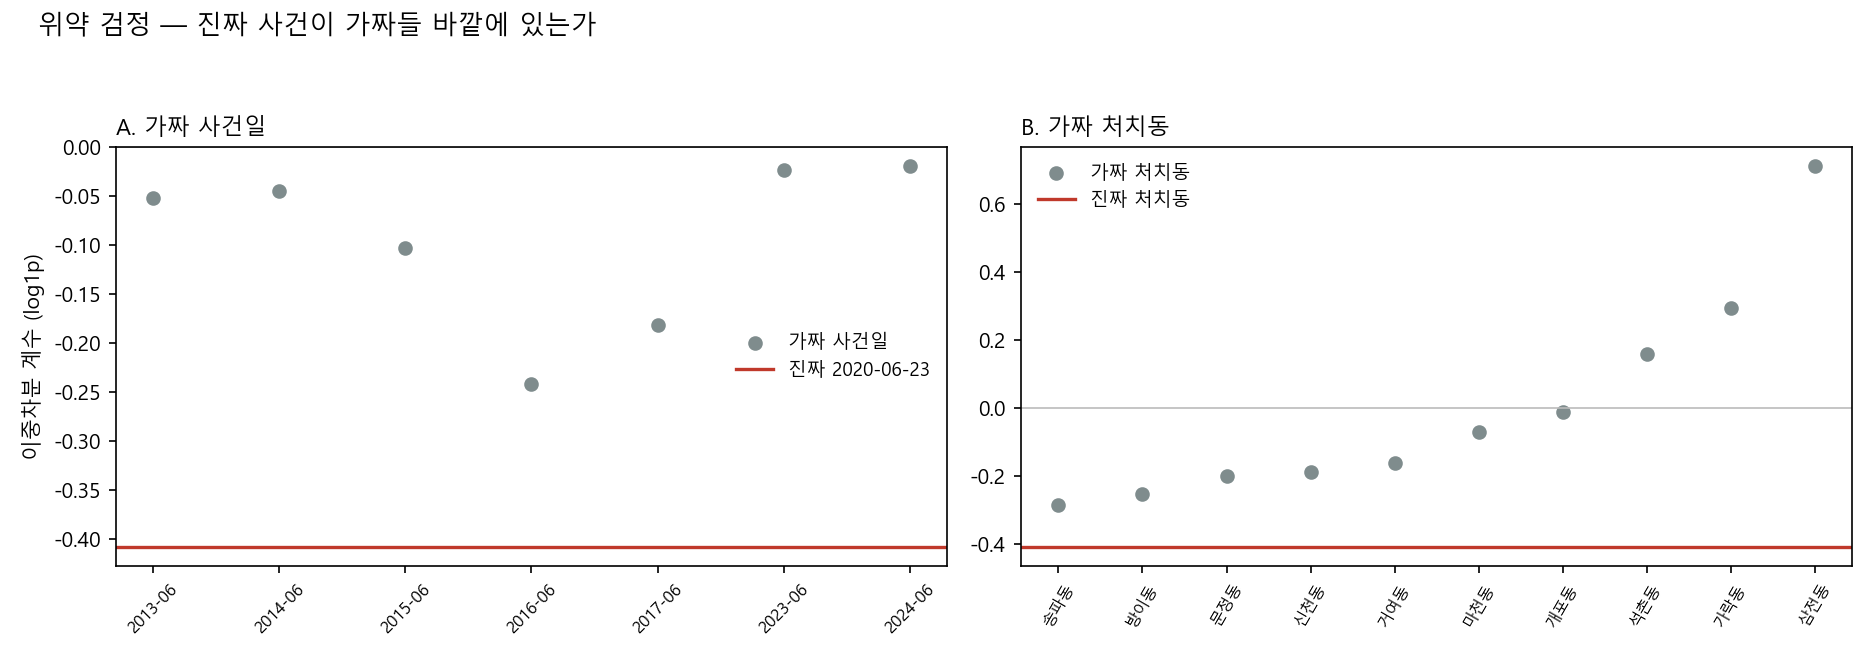
\includegraphics[width=\linewidth]{13_placebo.png}
  \caption{위약 검정. 왼쪽 가짜 사건일, 오른쪽 가짜 처치동.}
  \label{fig:placebo}
\end{figure}

\textbf{진짜가 가짜 최대($-21.5\%$)의 1.5배다. 그러나 가짜 둘이 유의하다.}
2016·2017년 창에는 \textbf{8·2 대책(2017-08)과 9·13 대책(2018-09)}이 들어 있고
둘 다 처치동에 더 크게 걸리는 규제다. \textbf{완전한 위약이 아니다.}

\textbf{가짜 처치동}으로도 돌렸다. 강남·송파 비처치동 23개 중 나중에 동 전체로
지정된 13개를 빼고 남은 10개를 처치군인 척 세우면 $-24.8\%$에서 $+103.5\%$까지
퍼지고, \textbf{진짜($-33.5\%$)가 그중 가장 크다.}

\textbf{그래서 0016의 결론은 ``효과는 있으나 크기는 구간으로 말한다''였다.}
24개월 효과를 단일 숫자로 쓰지 않는 이유의 하나다.

\subsection{합성대조군}

위약 검정이 숙제를 남겼다. 사전 거래량을 손으로 맞출수록 효과가 $-33.5\%$에서
$-24.8\%$로 줄고 유의성도 약해졌다 --- \textbf{평균 회귀가 섞였을 가능성을 배제하지
못했다.} 손으로 문턱을 정하는 방식은 문턱이 임의고, 표본을 버려 검정력도 잃으며,
사전 거래량으로 표본을 고르는 것 자체가 새로운 선택 편의를 만든다.

합성대조군은 \textbf{사전 궤적이 처치군과 가장 비슷해지도록 통제군의 가중평균을
자료가 직접 찾는다}\citep{abadie2010synthetic}. 문턱이 없고 표본을 버리지 않는다.

\begin{table}[htbp]
  \centering
  \caption{합성대조군 설계}
  \label{tab:scm-design}
  \begin{tabular}{ll}
    \toprule
    처치 단위 & 청담·삼성·대치·잠실을 합친 \textbf{하나} \\
    기증자 & 동 전체 지정 이력이 없고 사전 월평균 3건 이상인 서울 법정동
      \textbf{151개} \\
    결과변수 & $\log(1+\text{월 거래건수})$ $-$ 그 단위의 사전 36개월 평균 \\
    가중치 & 음수 아님, 합 1. 사전 36개월 궤적의 제곱오차 최소화 \\
    추론 & 배치 위약 --- 기증자 각각을 처치인 척 돌려 순위를 본다 \\
    \bottomrule
  \end{tabular}
\end{table}

\textbf{수준을 빼야 했다.} 처음에는 수준을 그대로 썼고 실패했다(사전 RMSPE 0.41,
경험적 $p$ 0.57). 처치 단위는 4개 동을 합쳐 월 210.9건인데 기증자 법정동은 중앙값
7.2건이다. \textbf{가중치가 음수가 아니고 합이 1이므로 볼록결합으로는 그 수준에
닿을 수 없다.} 단위별 사전 평균을 빼면 모두 0에서 출발해 궤적의 \emph{모양}만
맞추게 된다 --- 이중차분의 단위 고정효과와 같은 조작이다. 사전 RMSPE가 0.41에서
\textbf{0.17}로 떨어졌다.

\begin{figure}[htbp]
  \centering
  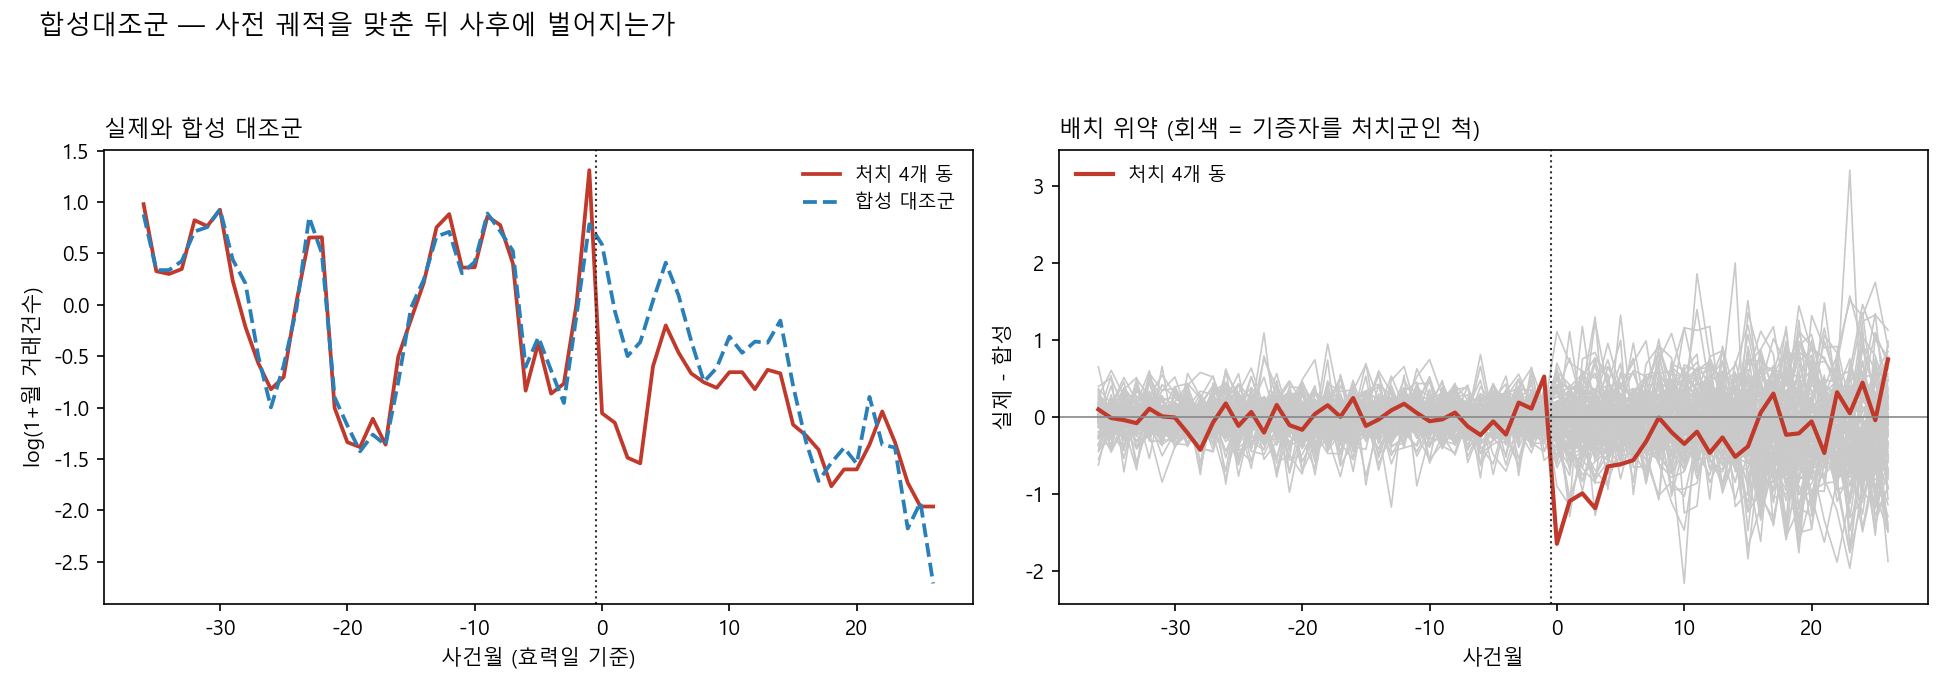
\includegraphics[width=\linewidth]{17_scm.png}
  \caption{합성대조군과 배치 위약. 빨간 선이 진짜 처치 단위, 회색이 기증자
           151개를 처치인 척 돌린 것이다.}
  \label{fig:scm}
\end{figure}

결과는 8.5절의 표~\ref{tab:scm-compare}에 있다. \textbf{지정 직후 3개월은 152개 중
1위($p=0.007$), 사후 27개월 평균은 22위($p=0.145$)다.} 사전 적합이 나쁜 가짜를
빼도(진짜의 2배 이내, 106개) 0.009와 0.206으로 같은 결론이다.

\textbf{통계량 선택의 순서를 밝힌다.} 사후 평균을 \emph{먼저} 돌렸고 유의하지
않았다. 그다음 직후 3개월로 바꾸어 유의한 값을 얻었다. 순서만 보면 사양 탐색이다.
다만 ``사후 $k \geq 4$는 해석하지 않는다''는 결정(0014)이 \textbf{이 분석보다 먼저}
있었고, 사후 27개월 평균은 그 해석하지 않기로 한 구간을 대부분 포함한다.
\textbf{둘 다 보고한다.}

\subsection{통제군 오염 제외}

강남·송파 통제동 23개 가운데 여섯이 분석 창 안에서 지정됐다(0009). 통제군이 일부
처치를 받으면 처치·통제 격차가 줄어 추정치가 0 쪽으로 끌린다(감쇠). 방향이
유리하다고 넘기지 않고 \textbf{이 동들을 뺀 사양을 함께 보고한다.}

\begin{table}[htbp]
  \centering
  \caption{창 안에 지정된 통제동 여섯}
  \label{tab:contam-list}
  \begin{tabular}{llrl}
    \toprule
    \textbf{동} & \textbf{지정 시작} & \textbf{사건월} & \textbf{방식} \\
    \midrule
    거여동 & 2021-04-04 & 9 & 혼합 \\
    압구정동 & 2021-04-27 & 10 & \textbf{동 전체} \\
    마천동 & 2022-01-02 & 18 & 혼합 \\
    송파동 & 2022-01-29 & 19 & 혼합 \\
    신천동 & 2022-01-29 & 19 & 혼합 \\
    일원동 & 2022-01-29 & 19 & 일부 \\
    \bottomrule
  \end{tabular}
\end{table}

\textbf{가장 이른 오염이 사건월 9다.} 지정 직후 3개월(사건월 0$\sim$2)에는 통제군
오염이 하나도 없다. 그러므로 직후 효과는 오염으로 줄어들 수 없다.

% 자동 생성 — scripts/build_tables.py. 손으로 고치지 않는다.
% 출처: output/results/13b_contamination.json : 결과
\begin{table}[htbp]
  \centering
  \caption{통제군 오염 동을 빼도 지정 직후 효과는 그대로다.}
  \label{tab:contamination}
  \begin{tabular}{lrrrr}
    \toprule
    \textbf{표본} & \textbf{법정동} & \textbf{효과 (\%)} & \textbf{WCR $p$} & \textbf{무작위화 순위} \\
    \midrule
    기본 & 27 & -79.8 & 0.014 & 1 \\
    압구정 제외 & 26 & -80.0 & 0.013 & 1 \\
    오염 6개 제외 & 21 & -80.0 & 0.008 & 1 \\
    \bottomrule
  \end{tabular}

  \begin{minipage}{\linewidth}\footnotesize
  \textit{주.} 가장 이른 오염이 사건월 9 다. 지정 직후 3개월에는 오염이 없다. 제외 목록은 결과를 보기 전(2026-09-07)에 정했다.
  \end{minipage}
\end{table}


\begin{figure}[htbp]
  \centering
  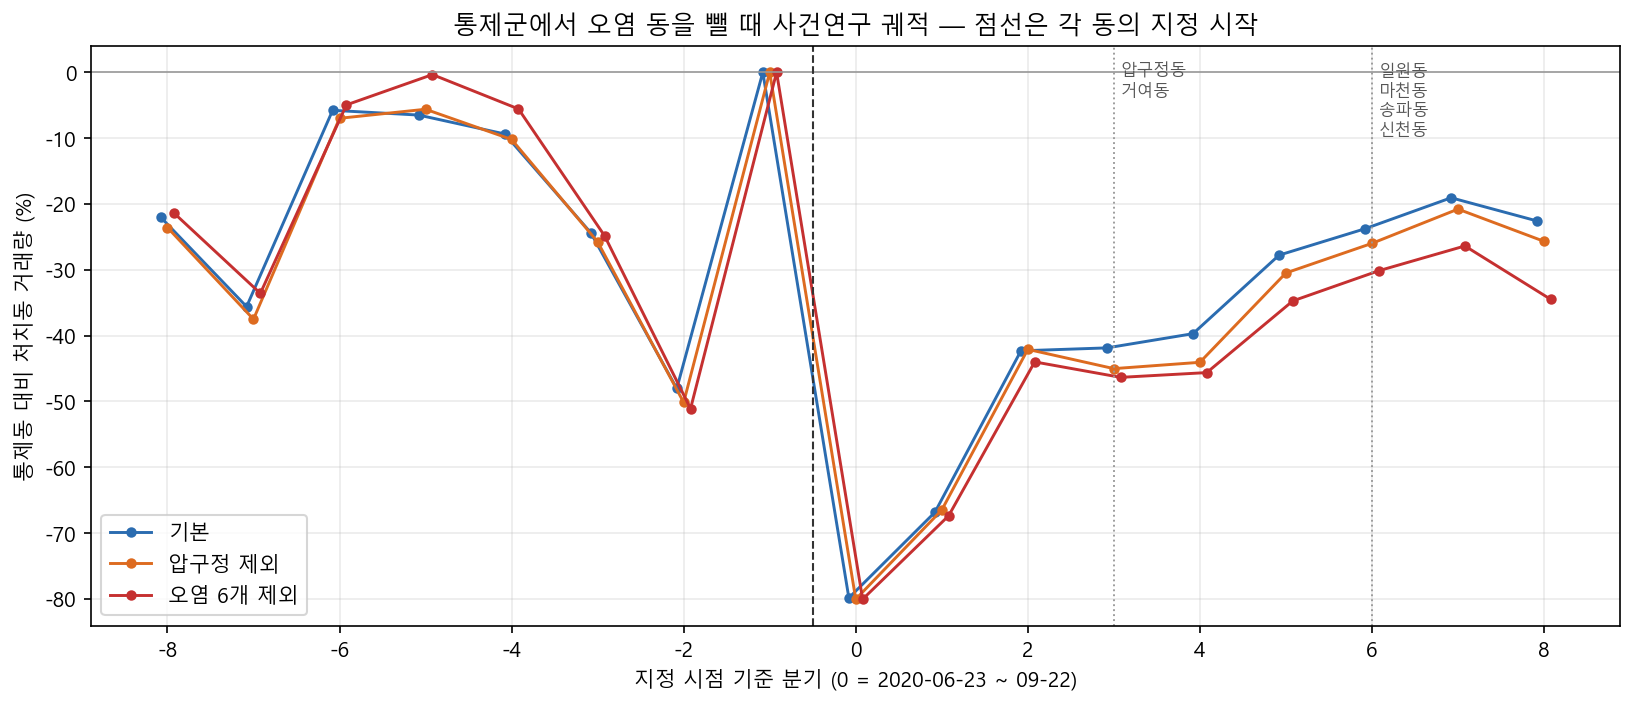
\includegraphics[width=\linewidth]{13b_contamination.png}
  \caption{오염 동을 뺄 때의 사건연구 궤적.}
  \label{fig:contamination}
\end{figure}

\textbf{직후 효과는 움직이지 않고($-79.8 \to -80.0\%$) 24개월 효과는 커진다}
($-33.5 \to -38.4\%$, WCR $p$ $0.047 \to 0.015$). 5.4절에서 ``24개월은 경계에
있다''고 적은 그 경계의 일부가 오염에 의한 감쇠였다. 모든 표본에서 무작위화
\textbf{1위}다.

\textbf{제외 목록은 결과를 보기 전에 정했다.} 0009가 2026-09-07에 목록을
확정했고 이 분석은 09-18에 했다. 결과를 보고 고른 표본이 아니다.

\subsection{처치 역전 --- 가중치와 $\text{DID}_M$}

제안서는 2025년 처치 역전 구간에 \citet{dechaisemartin2020twoway}의 비흡수 처치
추정량을 쓰겠다고 적었다. 그 약속의 이행이다(0027).

양방향 고정효과 추정량은 처치 효과가 이질적일 때 일부 칸에 \textbf{음의 가중치}를
줄 수 있다\citep{goodmanbacon2021}. 이미 처치된 집단이 다른 집단의 통제군 노릇을
하기 때문이다.

\textbf{표준적인 이질적 처치시점 추정량을 쓸 수 없는 이유를 먼저 적는다.}
\citet{callaway2021}와 \citet{sunabraham2021}은 처치가 한 번 시작되면
유지된다는 \textbf{흡수(absorbing) 가정}에 의존한다. 2025년 구간에서 A그룹의
처치 상태는 $1 \to 0 \to 1$로 전환되므로 그대로 적용할 수 없다. 그래서
비흡수 처치를 다루는 \citet{dechaisemartin2020twoway}의 $\text{DID}_M$을 쓴다.
합성 이중차분\citep{arkhangelsky2021}도 후보였으나, 처치 단위가 하나(4개 동을
합친 것)이고 역전 구간이 39일로 짧아 사전 적합에 쓸 구간이 부족해 쓰지 않았다.

\begin{table}[htbp]
  \centering
  \caption{TWFE 가중치 진단}
  \label{tab:dcdh-weights}
  \begin{tabular}{lrrr}
    \toprule
    \textbf{패널} & \textbf{처치 칸} & \textbf{음의 가중치} &
    \textbf{음의 가중치 합} \\
    \midrule
    \textbf{2020 주 분석} & 108 & \textbf{0개} & 0.000 \\
    2025 해제·재지정 & 5{,}350 & 675개 (12.6\%) & $-0.023$ \\
    \bottomrule
  \end{tabular}
\end{table}

\textbf{주 분석 패널에는 음의 가중치가 하나도 없다.} 2025 구간에도 합이 $-0.023$로
작다. $\text{DID}_M$으로 다시 재면 부과(재지정)가 $-43.0\%$
$[-50.8, -33.3]$, 해제가 $-28.2\%$ $[-58.9, +11.7]$이고 위약은 $+1.9\%$,
$-2.7\%$로 깨끗하다.

\begin{figure}[htbp]
  \centering
  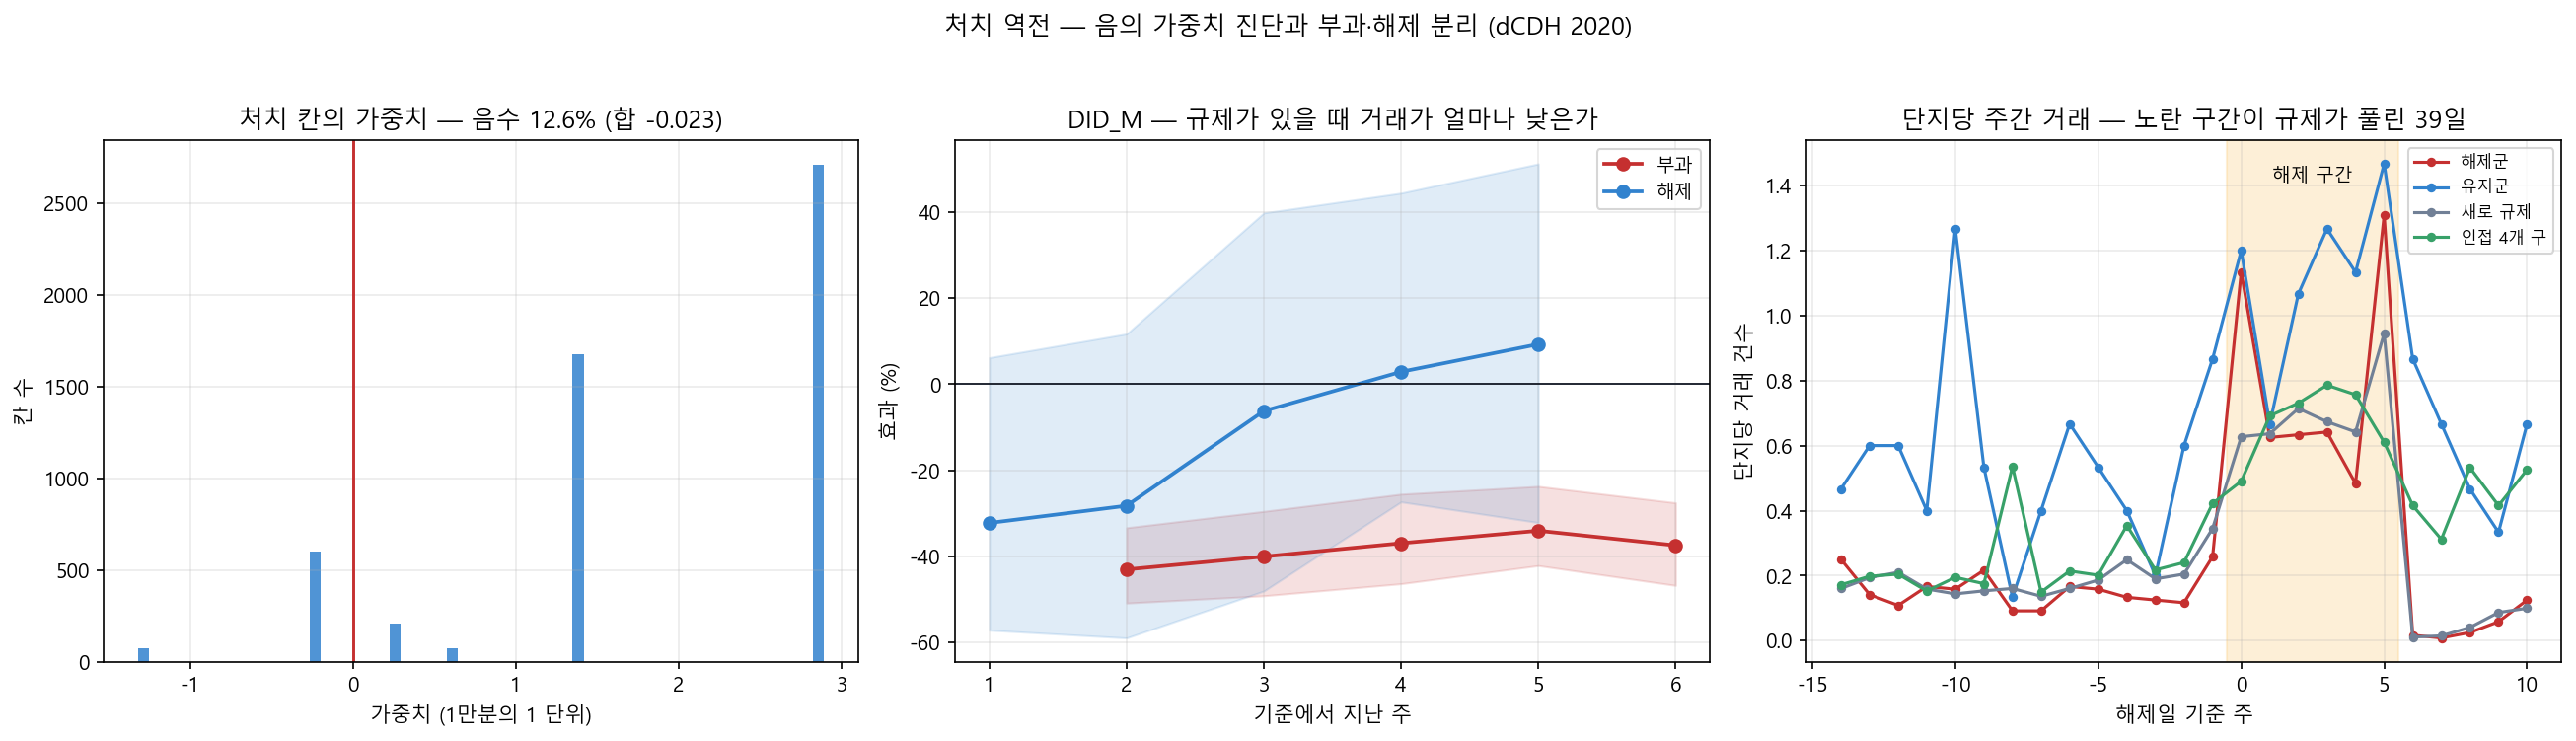
\includegraphics[width=\linewidth]{10_dcdh.png}
  \caption{TWFE 가중치 분포와 $\text{DID}_M$.}
  \label{fig:dcdh}
\end{figure}

\textbf{결론은 ``바꿀 필요가 없다''이다.} 그리고 \textbf{대칭성은 가릴 수 없다} ---
부과 쪽은 구간이 0을 품지 않고 해제 쪽은 품는다. 처음에는 ``처음 두 주만
대칭''이라고 썼다가, 막차 주간을 뺀 탓에 부과의 lag 0이 2주 변화였던 것을 발견해
\textbf{경과 주를 맞춰 다시 쟀다.} 결론이 바뀌었다.

\textbf{안 해 봤으면 몰랐다는 점이 결과다.}

\subsection{사양 곡선}

합리적인 설계 선택을 전부 조합했다(2.4절, 0028). 축과 조합 수는 그 절에 있다.

\begin{table}[htbp]
  \centering
  \caption{사양 곡선 요약}
  \label{tab:spec-summary}
  \begin{tabular}{lrr}
    \toprule
    & \textbf{거래량} & \textbf{가격} \\
    \midrule
    사양 수 & 192 & 144 \\
    중위 & $-68.9\%$ & $-5.3\%$ \\
    범위 & $-86.4 \sim -21.2\%$ & $-18.2 \sim \mathbf{+3.6\%}$ \\
    음수 & \textbf{100.0\%} & 79.9\% \\
    유의하게 음수 & \textbf{100.0\%} & \textbf{48.6\%} \\
    \bottomrule
  \end{tabular}
\end{table}

\begin{figure}[htbp]
  \centering
  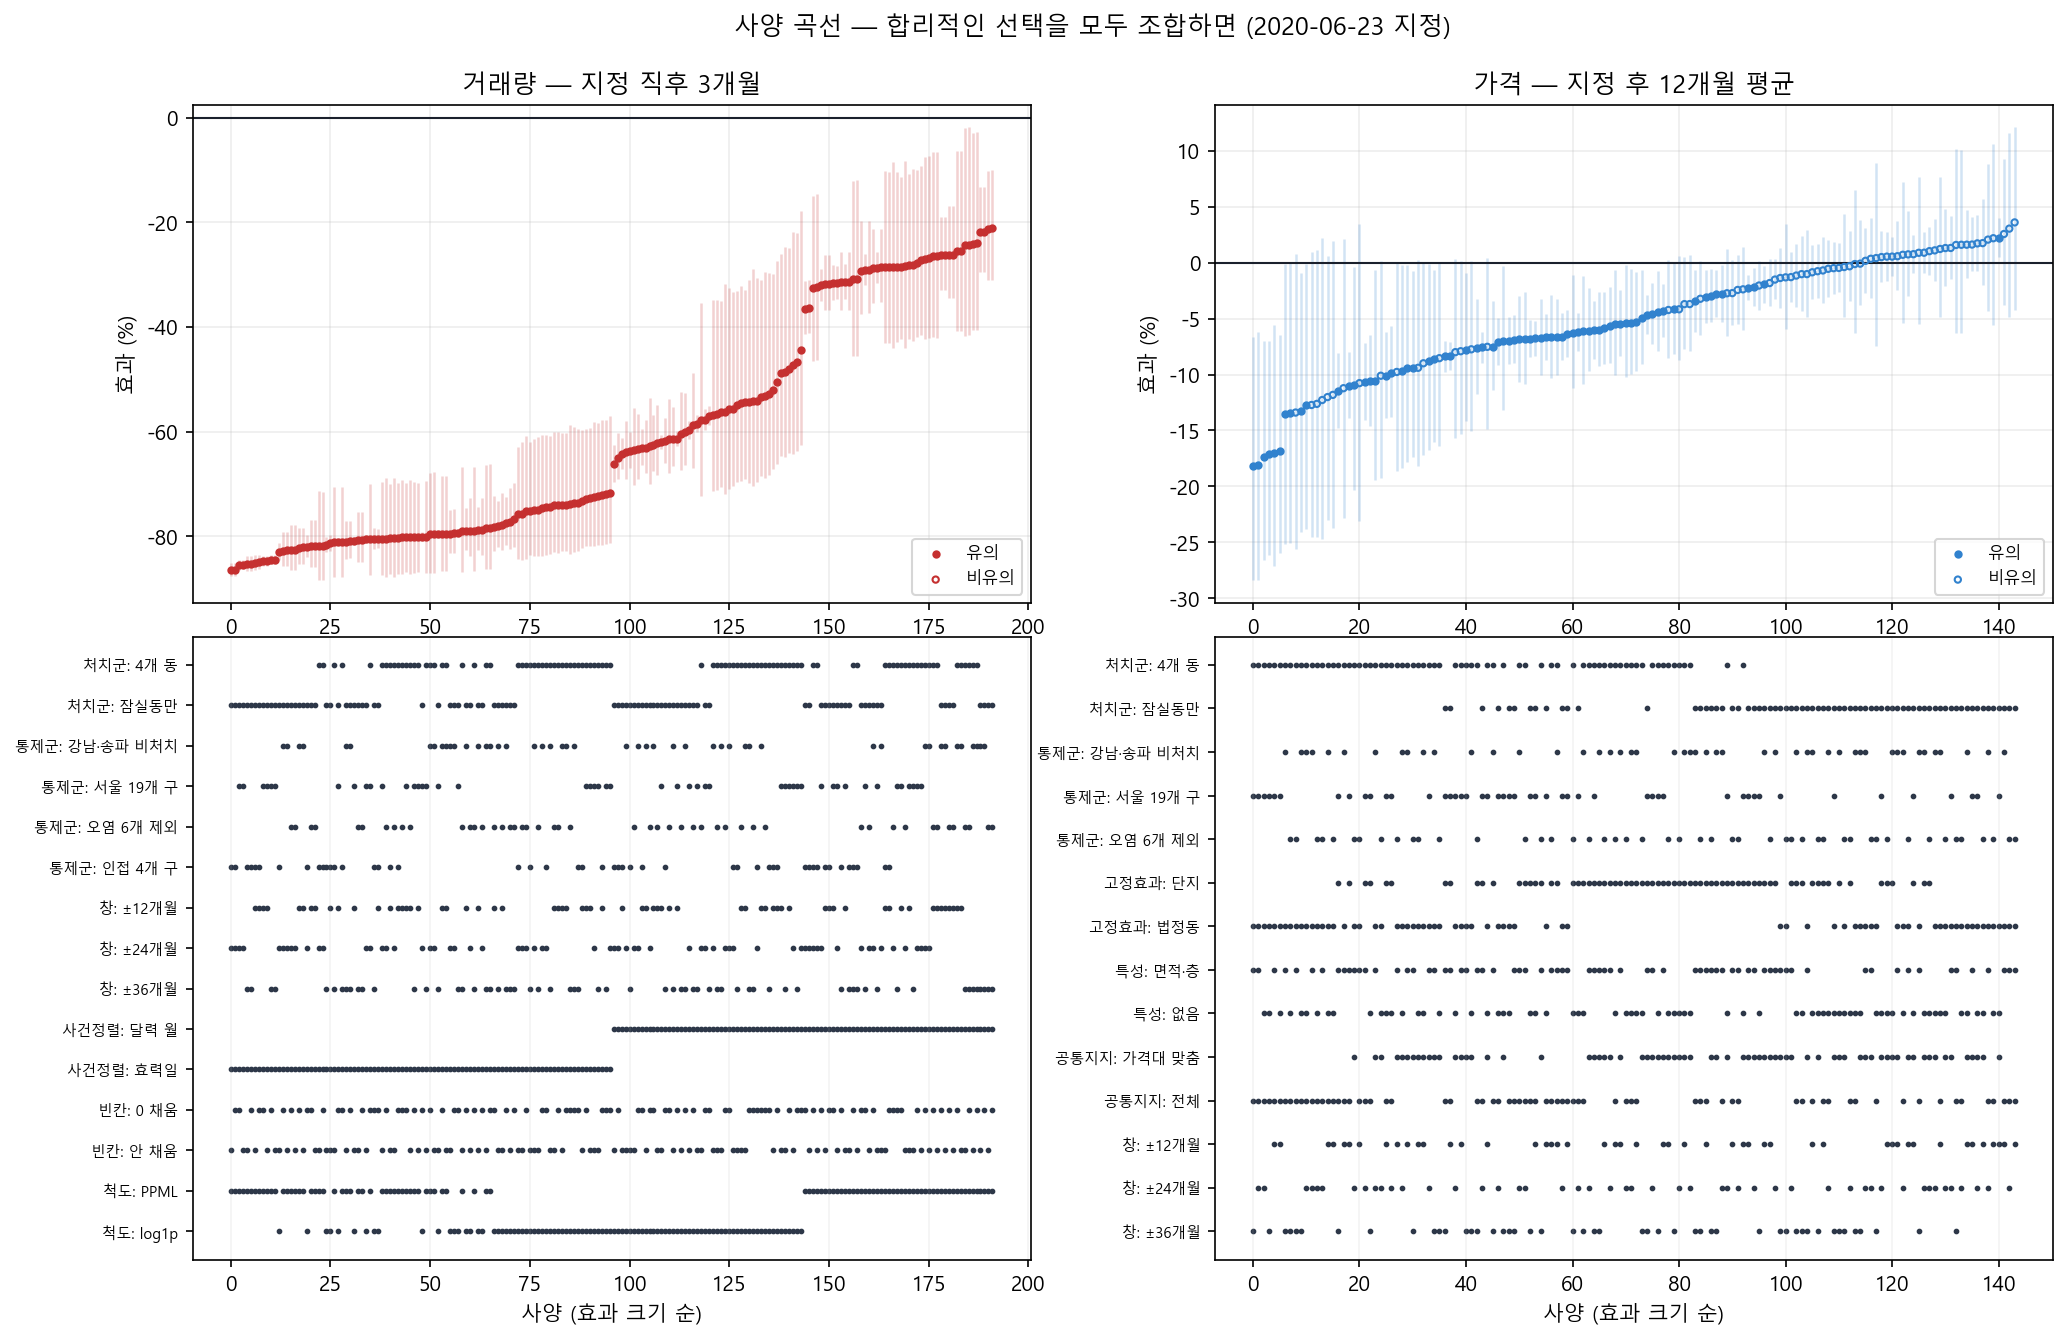
\includegraphics[width=\linewidth]{05b_spec_curve.png}
  \caption{사양 곡선. 점 하나가 설계 조합 하나로 추정한 효과이고, 아래 칸은 그
           조합이 어떤 선택을 썼는지다. 왼쪽 거래량 192, 오른쪽 가격 144.}
  \label{fig:spec-curve}
\end{figure}

\textbf{거래량은 192개가 전부 0 아래다.} 처치군을 잠실동 하나로 줄이든, 통제군을
서울 19개 구로 넓히든, 창을 $\pm$12에서 $\pm$36으로 늘리든, 달력 월로 세든, 빈칸을
안 채우든, 척도를 바꾸든 마찬가지다.

\textbf{다만 방향이 안 갈린다는 것은 당연한 쪽이다.} 거래에 허가를 붙였으니
줄어든다. \textbf{갈리는 것은 크기이고}($-21\%$에서 $-86\%$까지), 그래서 ``무엇이
그 차이를 만들었나''가 다음 질문이 되며 그 답이 2.4절의 축별 분해다.

\textbf{표준오차에 단서를 단다.} 사양 곡선의 $p$는 법정동 군집 관행값이다. 처치
동이 적은 사양에서는 이 $p$가 너무 작다(5.3절). \textbf{곡선은 점추정을 보는
그림이고 구간은 참고로만 읽는다.} ``192개 전부 유의''는 그래서 과대평가이고, 믿을
것은 \textbf{192개 전부 음수}라는 쪽이다.

\subsection{외적 타당성 --- 2021년 B그룹}

처치 동이 네 개뿐이다. 17,550가지 중 1위는 \textbf{``그 네 동이 우연이 아니다''일
뿐 ``다른 동에서도 그렇다''가 아니다.} 둘은 다른 주장이다.

2021년 4월 27일 지정된 B그룹(압구정·여의도·목동·성수동1가·2가)을 두 번째 사례로
걸었다(0031). \textbf{완전히 다른 네 자치구}(강남·영등포·양천·성동), 열 달 뒤의
사건이다.

\textbf{설계의 핵심은 대칭이다.} B그룹 숫자를 A그룹 숫자 옆에 그냥 놓으면 안 된다.
A는 같은 구 안(강남·송파)을 통제군으로 썼는데 B는 그럴 수 없다 --- 목동이 속한
\textbf{양천구에 쓸 수 있는 비지정 동이 0개}다. 차이가 지역 때문인지 통제군
때문인지 가릴 수 없게 된다. 그래서 둘을 했다.

\begin{enumerate}[leftmargin=2em, itemsep=2pt]
  \item \textbf{두 사건을 같은 통제군 정의(서울 전역 비지정)로 다시 잰다.}
        A의 주 사양($-79.8\%$)은 그대로 두고 이 재추정은 비교용이다.
  \item \textbf{두 패널을 쌓아 차이를 직접 추정한다}(stacked DID). 두 숫자를
        눈으로 견주면 `차이가 유의한가'를 말할 수 없다 --- 6.3절에서 같은 실수를
        하고 정정했다.
\end{enumerate}

통제군에서 창 안에 어떤 계열로든 지정된 동 77개, A그룹 처치동 4개와 맞닿은 동
14개, 상대 사건의 처치동, 창 안 거래 30건 미만을 뺐다. \textbf{B그룹 5개 동 중
3개(압구정·성수동1가·2가)가 A그룹 맞닿은 동}이므로 처치군을 둘로 나눠 돌렸다.

% 자동 생성 — scripts/build_tables.py. 손으로 고치지 않는다.
% 출처: output/results/21_b_group.json : 대칭
\begin{table}[htbp]
  \centering
  \caption{두 사건을 같은 자로. 같은 통제군 정의, 같은 창, 같은 추정량.}
  \label{tab:bgroup}
  \begin{tabular}{lrrrr}
    \toprule
    \textbf{사양} & \textbf{처치 동} & \textbf{효과 (\%)} & \textbf{WCR $p$} & \textbf{무작위화 $p$} \\
    \midrule
    A 2020.6 (처치 4개 동) & 4 & -49.2 & 0.038 & $<0.001$ \\
    B 2021.4 (처치 5개 동) & 5 & -44.7 & 0.057 & $<0.001$ \\
    B 2021.4 (목동·여의도만) & 2 & -46.2 & 0.136 & 0.001 \\
    \bottomrule
  \end{tabular}

  \begin{minipage}{\linewidth}\footnotesize
  \textit{주.} 창 전체($\pm$12개월) 이중차분이다. 늘 인용하는 $-79.8\%$ 는 지정 직후 3개월이라 재는 것이 다르다. 두 사건의 차이를 쌓아서 직접 추정하면 $+8.7\%$, 무작위화 $p=0.715$ 다.
  \end{minipage}
\end{table}


% 자동 생성 — scripts/build_tables.py. 손으로 고치지 않는다.
% 출처: output/results/21_b_group.json : 사다리
\begin{table}[htbp]
  \centering
  \caption{2021.4 B그룹 --- 기준점을 바꿔도 $-41.7 \sim -44.9\%$ 다.}
  \label{tab:ladder-b}
  \begin{tabular}{lrrrr}
    \toprule
    \textbf{기준점} & \textbf{동} & \textbf{효과 (\%)} & \textbf{WCR $p$} & \textbf{무작위화 $p$} \\
    \midrule
    ① 서울 전역 비지정 & 182 & -44.7 & 0.057 & $<0.001$ \\
    ② ① + 가격대 공통지지 & 39 & -41.7 & 0.063 & 0.002 \\
    ③ 오염 미제외 & 233 & -43.8 & 0.071 & $<0.001$ \\
    ④ A그룹 맞닿은 동 포함 & 188 & -44.9 & 0.063 & $<0.001$ \\
    \bottomrule
  \end{tabular}

  \begin{minipage}{\linewidth}\footnotesize
  \textit{주.} 목동이 속한 양천구에 쓸 수 있는 비지정 동이 0개라 `같은 구 안' 통제군을 주 사양으로 쓸 수 없었다.
  \end{minipage}
\end{table}


\begin{figure}[htbp]
  \centering
  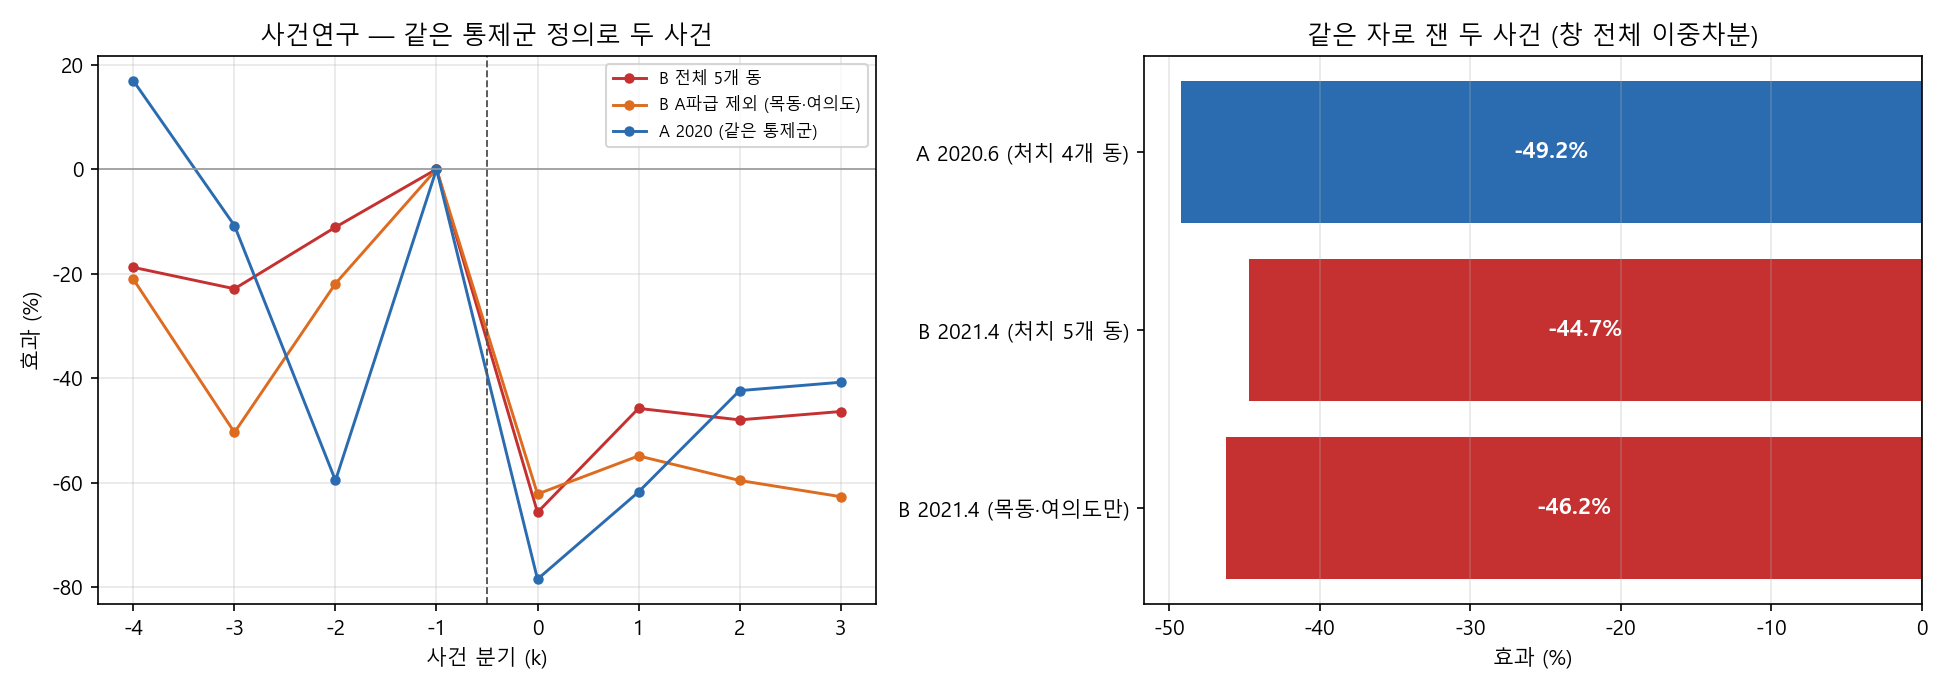
\includegraphics[width=\linewidth]{21_b_group.png}
  \caption{두 사건을 같은 자로. 왼쪽 사건연구, 오른쪽 창 전체 이중차분.}
  \label{fig:bgroup}
\end{figure}

\textbf{두 패널을 쌓아 차이를 직접 추정하면 $+8.7\%$, WCR $p$ 0.777, 무작위화
3{,}576/5{,}000($p=0.715$)다.} 0과 구분되지 않는다. \textbf{B가 A와 다르다고 할 수
없다.}

\textbf{덤으로 2.4절이 확인됐다.} A를 강남·송파 내부 통제로 재면 사건연구 $k=0$이
$-79.8\%$, 서울 전역 통제로 바꾸면 $-78.5\%$다. 사양 곡선이 통제군 축을 2.3\,\%p로
잰 것과 맞는다.

\textbf{면적 이질성은 B그룹에서 세울 수 없었다.} 2021년 지정의 허가 기준도 대지
18\,m$^2$이므로 메커니즘대로면 소형이 덜 줄어야 하고, 실제로 부호는 전부
양수다(40\,m$^2$에서 $+108.1\%$, $p=0.047$). 그러나 \textbf{40\,m$^2$ 미만 거래가
35건}(2020년은 322건)이고 경계를 올리면 유의성이 사라진다. 중위 전용면적은 A
84.8\,m$^2$ · B 85.0\,m$^2$로 같은데 40\,m$^2$ 미만 비중이 A 8.4\% 대 B
\textbf{1.2\%}다. \textbf{메커니즘의 반증이 아니라 검정력의 한계다.}

\textbf{B그룹 추정치를 주 결과로 올리지 않는다.} WCR이 0.057로 경계에 있고 기준분기
민감도도 A보다 넓다($-55.5 \sim -65.7\%$, 10\,\%p 폭 대 A의 7\,\%p). B는
\textbf{주 결과가 특정 지역의 산물이 아님을 보이는 보조 증거}다.

\subsection{자료 쪽 --- 취소거래}

마지막으로 \textbf{자료를 만들 때 뺀 것}이 결과를 바꾸는지 확인했다(0030).
3.3절에서 취소거래 6,293건을 뺐는데, 0004가 ``규제 직후에 몰린다면 그 자체가 정책
반응''이라는 숙제를 남겼었다.

% 자동 생성 — scripts/build_tables.py. 손으로 고치지 않는다.
% 출처: output/results/18_cancellations.json : 이중차분.2025-03-24 재지정
\begin{table}[htbp]
  \centering
  \caption{취소거래가 규제 직후에 몰리는가 (2025-03-24 재지정).}
  \label{tab:cancel}
  \begin{tabular}{lrrrrr}
    \toprule
    \textbf{창 (개월)} & \textbf{처치 전} & \textbf{처치 후} & \textbf{통제 전} & \textbf{통제 후} & \textbf{DID (\%p)} \\
    \midrule
    3 & 4.38 & 8.18 & 7.04 & 11.25 & -0.4 \\
    6 & 4.05 & 8.96 & 6.81 & 10.02 & +1.7 \\
    12 & 3.40 & 7.03 & 5.20 & 7.91 & +0.9 \\
    \bottomrule
  \end{tabular}

  \begin{minipage}{\linewidth}\footnotesize
  \textit{주.} 창을 바꾸면 부호가 바뀐다. 처치군 특유의 집중이 없다. 취소를 다시 넣어도 주 결과는 $0.3\%$p 움직인다.
  \end{minipage}
\end{table}


\begin{figure}[htbp]
  \centering
  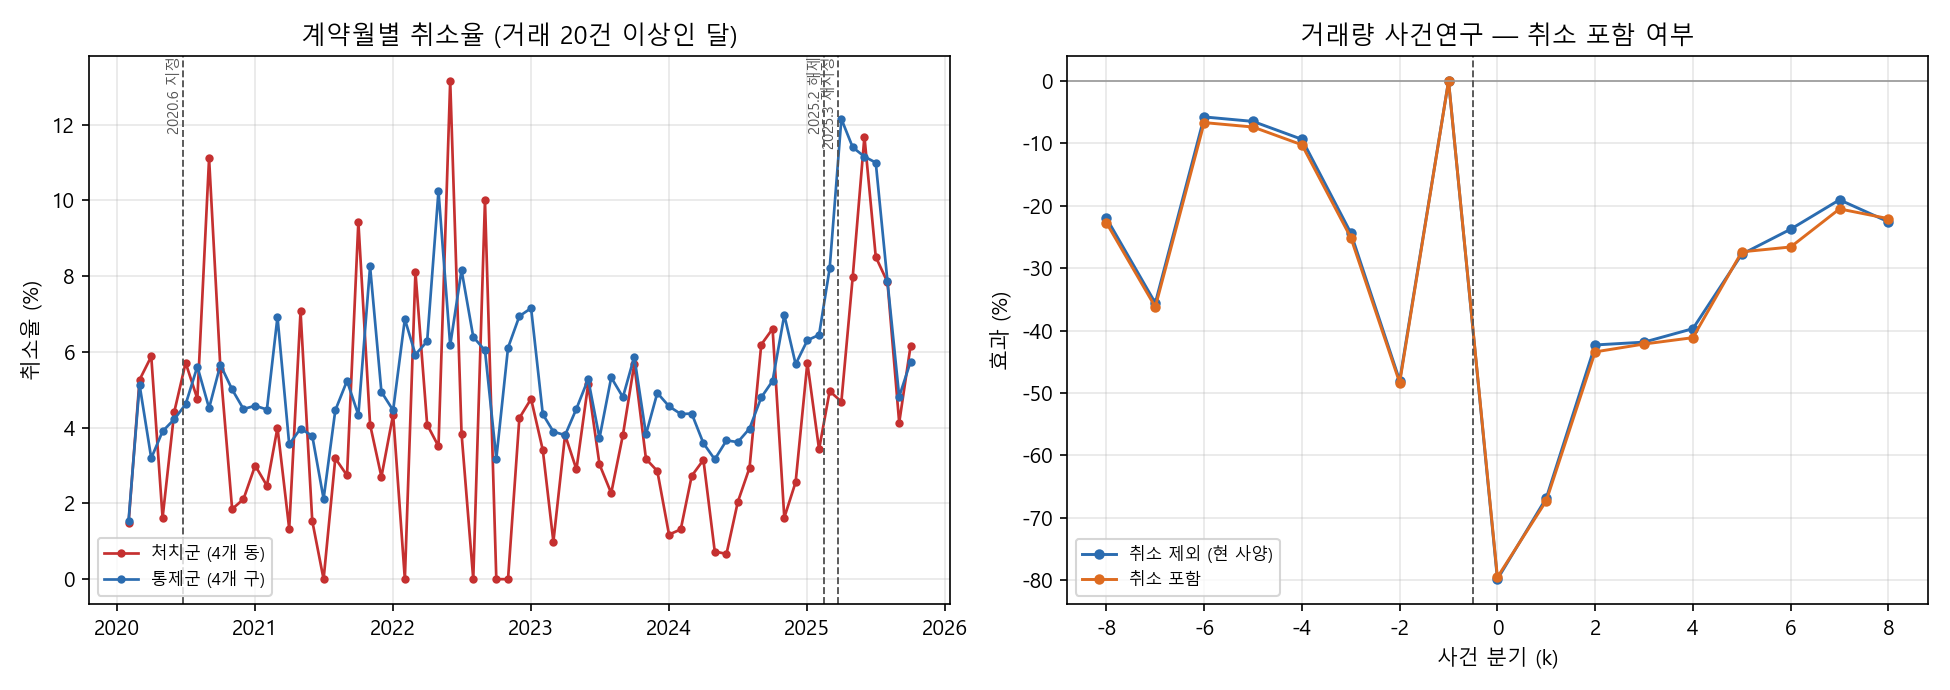
\includegraphics[width=\linewidth]{18_cancellations.png}
  \caption{취소거래의 시점별 분포. 왼쪽 계약월별 취소율, 오른쪽 취소를 넣은
           사건연구와 뺀 사건연구.}
  \label{fig:cancellations}
\end{figure}

\textbf{규제 직후에 몰리지 않는다.} 세 사건에 대해 취소율의 이중차분이 창에 따라
$-2.3 \sim +1.7$\,\%p로 부호가 바뀐다. 2025년에 양쪽 다 취소율이 오르는 것은 시장
전반의 일이고 처치와 무관하다.

\textbf{취소 거래가 더 비싸지도 않다.} 단지·계약월 고정효과 아래에서 취소 더미에
대한 $\log$ ㎡당가 회귀가 $-0.5\%$($p=0.443$)다. 허위신고 가설은 이 자료에서
지지되지 않는다.

\textbf{다시 넣어도 주 결과가 0.3\,\%p 움직인다}($-79.8 \to -79.5\%$). 취소율이
약 4\%이므로 사후 거래가 그만큼 깎이지만 \textbf{처치군과 통제군이 똑같이
깎이고} 이중차분은 공통된 비율 감소를 지운다.

\textbf{다만 취소 플래그는 2020년 2월 21일 계약분부터만 있다.} 2019년에 취소가
없었던 것이 아니라 자료에 없다. 이 비대칭을 처음에는 ``거래량 효과가 약 4\,\%p
부풀어 있다''고 적었다가, 재 보니 0.3\,\%p였다. \textbf{재지 않았으면 틀린 한계가
그대로 들어갔다.}
